\documentclass[conference]{IEEEtran}
\usepackage{cite}
\usepackage{amsmath,amssymb,amsfonts}
\usepackage{graphicx}
\usepackage{xcolor}
\usepackage{booktabs,tabularx,array}
\usepackage{tikz}
\usetikzlibrary{arrows.meta,positioning,calc}
\usepackage{url}
\usepackage[hidelinks]{hyperref}
\hypersetup{pdftitle={Autonomous Smart Dual Infusion and Patient Monitoring System Using ESP32},pdfauthor={MediSmart Project Team}}
\urlstyle{same}
\newcolumntype{Y}{>{\raggedright\arraybackslash}X}
\newcolumntype{P}[1]{>{\raggedright\arraybackslash}p{#1}}
\newcommand{\code}[1]{\texttt{\detokenize{#1}}}
\newcommand{\placeholder}[1]{\textit{[#1]}}
% Affiliation, supervisor, and repository were supplied by the user.
% Names and student IDs in the main file come from the presentation.
% City/country and author contact fields were removed at the user's request.
\newcommand{\ProjectDepartment}{BSCSE}
\newcommand{\ProjectUniversity}{United International University}
\newcommand{\ProjectSupervisor}{Arnab Bhattacharjee}
\newcommand{\ProjectAcknowledgment}{The authors thank their project supervisor, Arnab Bhattacharjee, for supervising this CSE 4326 project at United International University.}
\newcommand{\ProjectGithub}{\url{https://github.com/khalidhasan7343/CSE_4326_-Microprosser---Micro-controller-_Project}}
% The demonstration URL has not been supplied; retain the authorized placeholder.
% Replace the entire placeholder with \url{https://...} when available.
\newcommand{\ProjectYoutube}{\placeholder{ADD PROJECT YOUTUBE DEMONSTRATION URL}}

\graphicspath{{../Project_images/}{../Website_images/}{../medismart/}}
\hyphenation{MediSmart micro-controller data-base}

\begin{document}
\title{Autonomous Smart Dual Infusion and Patient Monitoring System Using ESP32}
\author{\IEEEauthorblockN{Md. Turjo Hasnat, Md. Khalid Hasan, Moieb Al Jawad,\\
Swarup Deb Nath, and Md Shakib}
\IEEEauthorblockA{Student IDs: 0112410067, 0112410009, 0112410289, 0112230150, 0112410546\\
\ProjectDepartment, \ProjectUniversity\\
Course: CSE 4326 --- Microprocessor and Microcontroller Project\\
Supervisor: \ProjectSupervisor}}
\maketitle

\begin{abstract}
Manual supervision of intravenous fluid delivery and separate bedside monitoring can make it difficult to coordinate fluid status, patient observations, and caregiver intervention. This project addresses that integration problem through an educational embedded prototype called MediSmart.
The implementation combines an ESP32 with a MAX30102 optical sensor, an AD8232 electrocardiogram front end, and an HX711 load-cell interface. Its firmware estimates pulse rate, oxygen saturation, and remaining fluid volume, drives saline, syringe, and oxygen-designated servo mechanisms, and controls a local buzzer. A Firebase Realtime Database connects device telemetry and control settings to doctor, patient, and family web interfaces.
The supplied photographs, source code, and dashboard captures document the assembled platform and a consistent 324.1~mL displayed/database fluid estimate with an open-valve state above a 320~mL stopping threshold. Measurement accuracy, actual delivered dose, end-to-end latency, power efficiency, and clinical suitability remain unquantified because the supplied materials contain no calibrated experimental dataset.
\end{abstract}
\begin{IEEEkeywords}
ESP32, intravenous monitoring, syringe actuation, MAX30102, AD8232, HX711, Firebase, embedded systems
\end{IEEEkeywords}

% Each file below is one chapter, rendered as an IEEE section to preserve
% the supplied conference format. See REPORT_INSTRUCTIONS.md for the rubric.
\section{Introduction}\label{sec:introduction}
\subsection{Problem Statement and Motivation}
Intravenous (IV) fluid delivery requires attention to the fluid source, the administration mechanism, and the patient's condition. In a manually supervised arrangement, a caregiver checks the container, adjusts the tubing or clamp, and separately observes vital signs. These activities motivate a common interface that reports fluid status and sensor availability while allowing supervised intervention. Research on remote infusion monitoring has explored optical drop detection and container-weight measurement to support this process~\cite{lee2021}.

The project presentation identifies manual IV and syringe operation, limited continuous monitoring, and repetitive caregiver tasks as the motivating problems. It also identifies affordability and suitability for resource-constrained hospitals in Bangladesh as design goals. These motivations describe the intended application; the provided materials do not contain a hospital deployment, stakeholder interview study, or measured reduction in caregiver workload.

MediSmart brings an IV stopping mechanism, a syringe mechanism, physiological sensing, and remote visualization onto a shared ESP32 platform. The engineering problem is to connect sensors with different interfaces, process their outputs, maintain actuator states, and exchange settings and telemetry over a network without blocking the local control sequence. The project is therefore relevant to microcontroller interfacing, digital signal processing, real-time task design, electromechanical actuation, and web-based monitoring.

\subsection{Objectives and Scope}
The implemented objectives are to estimate remaining fluid from a load-cell reading; acquire optical pulse and oxygen-saturation signals and an ECG analog signal; operate servo channels according to programmed conditions; activate a local buzzer during the firmware's low-oxygen condition; and expose monitoring/control views through Firebase. The term \emph{dual infusion} refers here to the saline and syringe mechanisms described by the project, rather than to two independently measured and calibrated infusion channels. A third servo channel is designated for an oxygen-related mechanism.

The scope of this report is the archived prototype. Source code establishes the programmed behavior, photographs establish visible construction, and screenshots establish captured interface states. None of these alone establishes calibrated volume delivery or safe therapeutic operation. Measured accuracy, actual response time, and energy efficiency are therefore identified as evaluation tasks rather than assigned numerical values.

\subsection{Literature Review}
Lee, Yoon, and Kim~\cite{lee2021} combined an optical sensor with a load cell for remote IV monitoring. Their system reports remaining fluid, infusion rate, and expected completion time to caregivers, and the study examines motion-related measurement limitations. This provides a useful comparison because MediSmart also uses container-weight information, but its archived implementation does not combine that reading with an optical drop counter or compute an infusion-rate estimate.

Contardi, Morikawa, Brunelli, and Thomaz~\cite{contardi2022} demonstrated a MAX30102 optical module connected to an ESP32 for remote heart-rate and oxygen-saturation monitoring. Their work supports the feasibility of integrating optical biosensing with a networked microcontroller. MediSmart extends that integration into a prototype that also includes ECG acquisition, fluid estimation, and servo mechanisms; this difference does not demonstrate superior physiological measurement accuracy.

Kok and colleagues~\cite{kok2024} developed a cloud-connected infusion platform with remote supervision through Blynk. Their design includes a stepper-driven pumping mechanism and infusion-related sensing, illustrating the importance of observing delivery as well as commanding a motor. MediSmart instead uses Firebase and three PWM servo channels in the archived firmware. Its saline threshold and syringe motion sequence are simpler than a calibrated infusion-rate controller.

Table~\ref{tab:related} summarizes the features relevant to this project. The comparison concerns the cited implementations and the supplied MediSmart archive; it is not a performance benchmark.
\begin{table*}[!t]
\caption{Feature Comparison with Selected Published Work}\label{tab:related}
\centering\small
\begin{tabularx}{\textwidth}{@{}P{0.19\textwidth}YYY@{}}
\toprule
Work & Main sensing and mechanism & Communication and interface & Relation to MediSmart \\
\midrule
Lee, Yoon, and Kim~\cite{lee2021} & Optical drop detection and load-cell monitoring & Remote IV information and notifications & Provides a multisensor comparison; MediSmart's current fluid estimate uses HX711/load-cell input only. \\
Contardi and colleagues~\cite{contardi2022} & MAX30102 pulse and oxygen-saturation sensing with ESP32 & Remote physiological visualization & Shares the optical sensing/controller combination; MediSmart also incorporates fluid and actuator functions. \\
Kok and colleagues~\cite{kok2024} & Stepper-driven infusion and delivery-related sensors & Blynk web/mobile supervision & Provides an alternative cloud and pumping architecture; MediSmart implements servo motion and Firebase settings. \\
MediSmart archive & MAX30102, AD8232, HX711; saline, syringe, and oxygen-designated servos & Shared Firebase telemetry and doctor/patient/family views & Integrates the functions in one educational prototype; calibrated delivery and physiological accuracy are unverified. \\
\bottomrule
\end{tabularx}
\end{table*}

\subsection{Project Contributions and Distinguishing Features}
The project's contribution is the integration of fluid estimation, physiological acquisition, local actuation, and several caregiver-facing views. The doctor interface changes the remaining-volume rules and displays device-reported valve and syringe states. The patient and family interfaces provide simpler pulse/oxygen displays, with an on-page family alert for programmed conditions. A separate network task exchanges settings while local firmware evaluates the actuator conditions.

These are distinguishing features of this prototype relative to the selected examples, rather than claims that no previous project has implemented them. The archived design also differs from the early presentation: load-cell sensing, AD8232 acquisition, and an oxygen-designated servo appear in the code and wiring; a stepper driver sequence, LCD driver, IR drop-counting routine, and ESP-NOW link do not. Subsequent chapters describe the implementation that can be traced to the supplied evidence.


\section{Proposed Method}\label{sec:method}
\subsection{Block Diagram of the Overall System}
Fig.~\ref{fig:architecture} presents the implemented signal and control paths. Three sensing inputs feed the ESP32: the MAX30102 supplies red/infrared optical samples over I\textsuperscript{2}C, the AD8232 supplies an analog ECG signal and lead-off indications, and the HX711 supplies digitized load-cell data. The controller processes the samples and drives three servo channels and a buzzer. Wi-Fi connects a separate firmware task to Firebase, which stores current telemetry and remote settings.

\begin{figure*}[!t]
\centering
\resizebox{\textwidth}{!}{%
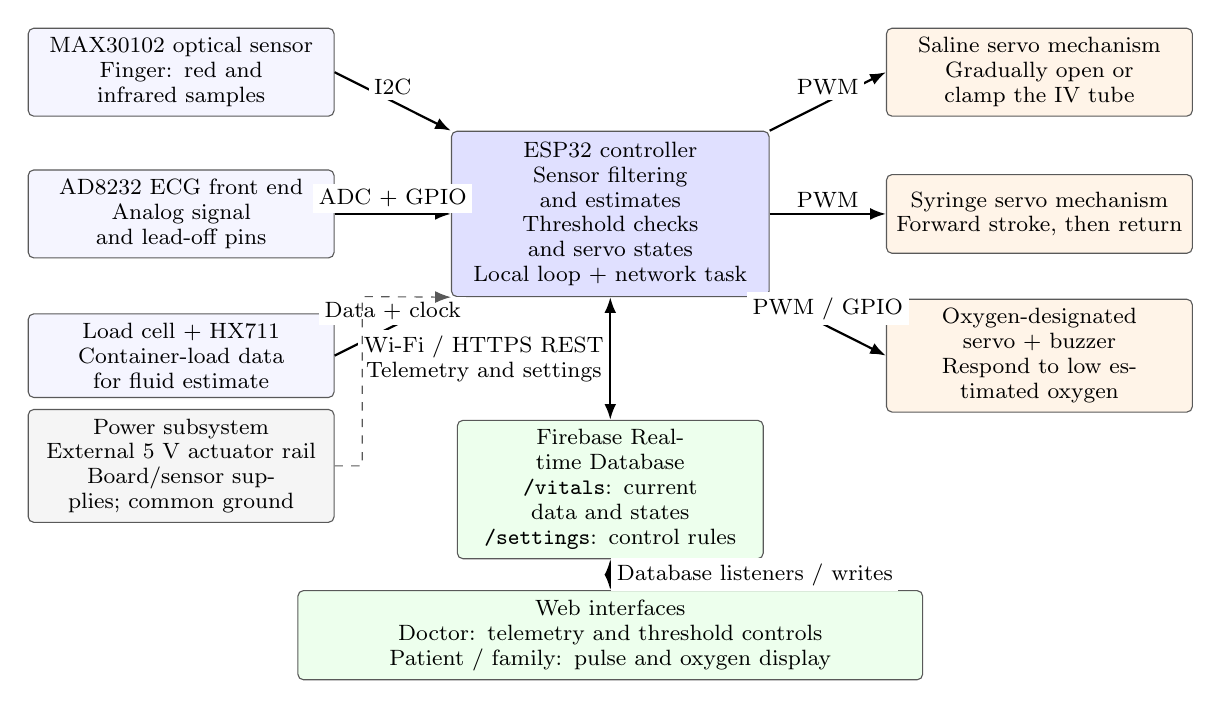
\begin{tikzpicture}[x=1cm,y=1cm,
 box/.style={draw=black!65,rounded corners=2pt,fill=blue!4,align=center,text width=3.65cm,minimum height=1.0cm,font=\fontsize{8}{9}\selectfont},
 control/.style={box,fill=blue!12,text width=3.8cm,minimum height=2.1cm},
 actuator/.style={box,fill=orange!9},
 flow/.style={-{Latex[length=2mm]},thick},
 power/.style={-{Latex[length=2mm]},dashed,black!65},
 lab/.style={font=\fontsize{8}{9}\selectfont,fill=white,inner sep=2pt,align=center}]
\node[box] (ppg) at (0,0) {MAX30102 optical sensor\\Finger: red and infrared samples};
\node[box] (ecg) at (0,-1.8) {AD8232 ECG front end\\Analog signal and lead-off pins};
\node[box] (load) at (0,-3.6) {Load cell + HX711\\Container-load data for fluid estimate};
\node[control] (esp) at (5.45,-1.8) {ESP32 controller\\Sensor filtering and estimates\\Threshold checks and servo states\\Local loop + network task};
\node[actuator] (saline) at (10.9,0) {Saline servo mechanism\\Gradually open or clamp the IV tube};
\node[actuator] (dose) at (10.9,-1.8) {Syringe servo mechanism\\Forward stroke, then return};
\node[actuator] (o2) at (10.9,-3.6) {Oxygen-designated servo + buzzer\\Respond to low estimated oxygen};
\node[box,fill=green!7] (cloud) at (5.45,-5.3) {Firebase Realtime Database\\\texttt{/vitals}: current data and states\\\texttt{/settings}: control rules};
\node[box,text width=7.7cm,fill=green!7] (web) at (5.45,-7.15) {Web interfaces\\Doctor: telemetry and threshold controls\\Patient / family: pulse and oxygen display};
\node[box,fill=gray!8] (supply) at (0,-5.0) {Power subsystem\\External 5 V actuator rail\\Board/sensor supplies; common ground};
\draw[flow] (ppg.east) -- (esp.north west) node[midway,lab,above] {I2C};
\draw[flow] (ecg.east) -- (esp.west) node[midway,lab,above] {ADC + GPIO};
\draw[flow] (load.east) -- (esp.south west) node[midway,lab,above] {Data + clock};
\draw[flow] (esp.north east) -- (saline.west) node[midway,lab,above] {PWM};
\draw[flow] (esp.east) -- (dose.west) node[midway,lab,above] {PWM};
\draw[flow] (esp.south east) -- (o2.west) node[midway,lab,above] {PWM / GPIO};
\draw[flow,{Latex[length=2mm]}-{Latex[length=2mm]}] (esp.south) -- (cloud.north) node[midway,lab,left] {Wi-Fi / HTTPS REST\\Telemetry and settings};
\draw[flow,{Latex[length=2mm]}-{Latex[length=2mm]}] (cloud.south) -- (web.north) node[midway,lab,right] {Database listeners / writes};
\draw[power] (supply.east) -- (2.3,-5.0) -- (2.3,-2.85) -- (esp.south west);
\end{tikzpicture}}
\caption{Overall implementation architecture reconstructed from the firmware, website, and supplied wiring diagrams. Power connections are summarized; the separate wiring diagrams show the detailed rails. Servo arrows indicate commands, without measured flow or position feedback.}\label{fig:architecture}
\end{figure*}

\subsection{Function of Each Subsystem}
\subsubsection{Controller and Local Scheduling}
The ESP32 is configured as a Wi-Fi station. Its main loop reads sensors, calculates conditions, updates servo angles, and prints diagnostics. A FreeRTOS task performs Firebase HTTP requests separately. The main loop ends with a 20~ms delay, while the network task ends with a 2000~ms delay; actual periods also include computation, sensor waiting, request duration, and scheduling.

The network task obtains \code{/settings.json} with GET and updates \code{/vitals.json} with PATCH. This separates the slower network exchanges from the actuator sequence, but shared variables are not protected by a snapshot or mutex. The design is a single-device implementation: the database paths do not include a patient or device identifier.

\subsubsection{Optical Pulse and Oxygen Estimation}
The MAX30102 contains red/infrared optical sensing and a digital interface~\cite{max30102}. The firmware uses I\textsuperscript{2}C address \code{0x57} at 100~kHz and reads six FIFO bytes per loop to reconstruct the two 18-bit values. An infrared value below 20000 clears the reported pulse and oxygen values, representing no detected usable finger signal.

For a valid optical input, a running DC estimate for channel sample $x[n]$ is
\begin{equation}
D[n]=0.95D[n-1]+0.05x[n],\qquad A[n]=x[n]-D[n].
\end{equation}
The pulse routine detects an infrared AC threshold crossing followed by a decreasing sample. It imposes an interval greater than 400~ms between accepted beat events and calculates
\begin{equation}
\mathrm{BPM}_{\mathrm{candidate}}=\frac{60000}{\Delta t_{\mathrm{ms}}}.
\end{equation}
Only candidates strictly between 50 and 130~BPM enter an eight-value buffer. Once at least five values exist, the routine sorts them, removes the smallest and largest, and averages the remainder. The displayed estimate applies additional smoothing with coefficients 0.97 and 0.03. These choices reduce visible variation but delay changes and exclude pulse rates outside the acceptance range.

The oxygen estimate uses peak-to-peak AC amplitudes and DC levels:
\begin{equation}
R=\frac{A_{\mathrm{red,pp}}/D_{\mathrm{red}}}{A_{\mathrm{IR,pp}}/D_{\mathrm{IR}}},\qquad
S_{\mathrm{candidate}}=110-25R.
\end{equation}
The candidate is restricted to 80--100\%, then smoothed as $S[n]=0.9S[n-1]+0.1S_{\mathrm{candidate}}$ after initialization. These are the implemented algorithm and output limits, not verified oxygen-saturation accuracy. The archive supplies no reference-device comparison or calibration record.

\subsubsection{ECG Acquisition}
The AD8232 is a single-lead signal-conditioning front end designed to interface with an ADC~\cite{ad8232}. Its output feeds ESP32 ADC1 channel~6 on GPIO~34; LO+ and LO$-$ feed GPIO~25 and GPIO~26. If either lead-off input is high, the firmware sets the ECG value to zero. Otherwise it reads one raw ADC sample. The web chart receives only the latest cloud-published sample and therefore does not reproduce the complete locally acquired waveform.

\subsubsection{Load-Cell Fluid Estimate}
The HX711 serial interface is read through data and clock GPIOs. After the firmware's 24-bit conversion, a nonzero transformed count $W[n]$ is mapped to the nonnegative fluid proxy
\begin{equation}
V_{\mathrm{raw}}[n]=\max\!\left(0,\frac{W[n]-8388608}{1000}\right).
\end{equation}
When the stored estimate is zero, the new value is adopted directly; otherwise the update is
\begin{equation}
V[n]=0.85V[n-1]+0.15V_{\mathrm{raw}}[n].
\end{equation}
The firmware and dashboard express $V$ in mL. A physical weight-to-volume measurement also requires a documented tare, calibration factor, mounting condition, and fluid-density assumption. Since these are absent, this report describes $V$ as a remaining-fluid estimate or proxy rather than a calibrated volume measurement. A timeout retains the previous estimate without an explicit invalid-data flag.

\subsection{Actuator Rules and Motion Sequences}
Three LEDC channels share a 50~Hz, 13-bit PWM timer. The ideal angle-to-pulse relation for servo angle $\theta$ is
\begin{equation}
t_p(\theta)=500+\frac{2000\theta}{180}\quad (\mu\mathrm{s}),\qquad 0\leq\theta\leq180.
\end{equation}
The nominal frame duration is 20000~$\mu$s. The implementation uses integer division for the pulse-width term and then quantizes duty to the timer's resolution. Commanded angle is the software state; no external position sensor establishes the mechanical angle.

\subsubsection{Saline Stopping Rule}
For configured threshold $T_s$, the clamp condition is
\begin{equation}\label{eq:saline}
C_s=(T_s>0)\land(V<T_s).
\end{equation}
When true, the saline angle increases by $2^{\circ}$ per loop toward $180^{\circ}$ and the reported state progresses from \emph{Closing} to \emph{Stopped}. Otherwise the angle decreases by $2^{\circ}$ toward zero and the state progresses from \emph{Opening} to \emph{Open}. Equality does not initiate closing. This is a remaining-volume stop rule; it does not command a continuous infusion rate in mL/h.

\subsubsection{Syringe Sequence}
For threshold $T_d$, the volume-based condition is $(T_d>0)\land(V<T_d)$. The firmware also checks whether the current local hour and minute match \code{dose_time}, if such a setting has been parsed. Either condition starts a cycle when no cycle is active. The servo advances by $1^{\circ}$ per loop toward $180^{\circ}$, reports \emph{Pushing}, then requests a cloud reset of \code{dose_trigger_ml} and returns by $2^{\circ}$ per loop toward zero. The final state is \emph{Standby}.

No programmed syringe volume, plunger-position measurement, or flow calibration is supplied. The web reset button clears a trigger value and does not implement an immediate abort of an active cycle. The time condition has no once-per-event latch, so additional cycles can start while the matching minute remains active. These limitations are considered in Section~\ref{sec:discussion}.

\subsubsection{Oxygen-Designated Servo and Buzzer}
The local condition is $0<S<85\%$. When true, the firmware sets the buzzer GPIO high and advances the oxygen-designated servo by $2^{\circ}$ per loop. Otherwise it silences the buzzer and returns the servo toward zero. The 85\% value is a project constant and is not presented as a clinically approved treatment threshold. The photographs include a mask and tubing, but no oxygen-flow sensor or measured delivery result establishes the mechanism's therapeutic effect.

\subsection{Cloud Data and Web Interfaces}
Table~\ref{tab:schema} lists the active cloud fields. The doctor page listens for telemetry and settings changes, plots a rolling buffer of 50 received ECG values, and writes two fluid thresholds. Its open button sets $T_s=0$; its close button sets $T_s=9999$, making the clamp condition true when the estimated volume is below that sentinel. The reset button sets $T_d=0$.

\begin{table}[!t]
\caption{Implemented Firebase Data Contract}\label{tab:schema}
\centering\footnotesize
\begin{tabularx}{\columnwidth}{@{}P{0.20\columnwidth}YY@{}}
\toprule
Path & Fields & Purpose \\
\midrule
\code{/vitals} & \code{bpm}, \code{spo2}, \code{ecg}, \code{current_ml} & Latest processed estimates and raw ECG sample. \\
\code{/vitals} & \code{saline_status}, \code{dose_status} & Software-reported servo sequence states. \\
\code{/settings} & \code{saline_stop_ml}, \code{dose_trigger_ml} & Remaining-volume control thresholds. \\
\code{/settings} & \code{dose_time} & Firmware-only hour/minute trigger; no corresponding web control. \\
\path{/users/<uid>} & \code{email}, \code{role} & Registration record used for login routing. \\
\bottomrule
\end{tabularx}
\end{table}

Registration uses Firebase email/password authentication and stores a selected patient, family, or doctor role. Login reads this role to select a page. Patient and family pages include a signed-in check; the archived doctor page lacks an authentication guard and retains configuration placeholders. Therefore the report distinguishes role-based page routing from verified role-based authorization, which requires server-enforced access rules~\cite{firebaserules}.

The patient view labels a zero reading as \emph{Sensor Ready / Place Finger}. The family view displays an alert for BPM above 120, positive BPM below 50, or positive SpO\textsubscript{2} below 92\%. The doctor view uses positive SpO\textsubscript{2} below 85\% for its oxygen warning and interprets an ECG value of zero as lead disconnection. These inconsistent prototype display thresholds are documented rather than reconciled by assuming a common medical policy.


\section{Implemented Hardware System}\label{sec:hardware}
\subsection{Hardware Equipment and Model Identification}
Table~\ref{tab:hardware} records the hardware supported by the firmware, wiring sketches, and photographs. Exact model information is retained where documented, and ambiguous identities are marked for confirmation. The photographed load cell has a readable 5~kg label, while the ESP32 development-board variant and power-source rating are not established by readable labels.

\begin{table*}[!t]
\caption{Hardware Inventory and Evidence of Component Identity}\label{tab:hardware}
\centering\small
\begin{tabularx}{\textwidth}{@{}P{0.22\textwidth}P{0.23\textwidth}Y@{}}
\toprule
Equipment & Model / specification & Role and evidence \\
\midrule
Microcontroller development board & ESP32; PlatformIO target \code{esp32dev} & Main acquisition, actuation, Wi-Fi and task scheduling. Exact board/module variant requires confirmation. \\
Optical biosensor module & MAX30102 & Red/infrared acquisition for pulse and SpO\textsubscript{2} estimates; named in code, slides, and sensor wiring. \\
Single-lead ECG front end & AD8232 & Analog signal conditioning and lead-off outputs; named in the sensor wiring, with matching firmware pins. \\
Load-cell ADC/interface & HX711 & Reads the container-load sensor; identified by firmware and wiring. \\
Load cell and hook & 5~kg capacity label; exact part number unspecified & Upper stand assembly visible in photograph~4. Mechanical mounting converts supported load to a sensing input. \\
Saline clamp servo & SG90 in wiring; MG996R in code comments & PWM output on GPIO~5. Physical model must be confirmed because the two sources disagree. \\
Syringe and oxygen-designated servos & MG996R in wiring and code comments & PWM outputs on GPIO~18 and GPIO~16. Actual torque/travel and delivered quantities were not measured in supplied records. \\
Local alarm & Active buzzer; exact part number unspecified & GPIO~4 output, named in the actuator diagram and firmware. \\
Syringe mechanism & Syringe, handmade guide, rack and gear & Photographed mechanism; syringe capacity and travel-to-volume calibration are unspecified. \\
Fluid/oxygen-related assembly & Tubing, mask, and mounted mechanical components & Visible in photographs~2, 3, and 6; exact regulator/container ratings and output flow are unspecified. \\
Structure and power & Pole, caster base, enclosure, breadboards, wiring; external 5~V actuator rail in diagram & Provides physical integration. Battery chemistry, capacity, regulator identity, and current budget require confirmation. \\
Additional photographed hardware & Motor-driver-like board, secondary controller, ultrasonic-style modules & Visible in photographs but not operated by the supplied ESP32 source. Exact models and any separate mobility firmware are unspecified. \\
\bottomrule
\end{tabularx}
\end{table*}

The presentation additionally lists an IR drop sensor, stepper motor, lead screw, LCD, rechargeable battery, and following sensor/camera. The supplied medical firmware contains no corresponding drop-counting, stepper, LCD, or following-control routines. These items are not presented as verified functioning modules in the implementation inventory.

\subsection{Electrical Interfacing and Pin Assignment}
Table~\ref{tab:pins} gives the code/wiring pin assignment. The MAX30102 communicates through SDA and SCL; the AD8232 provides an ADC input and two digital status inputs; and the HX711 uses a clock/data interface. The three servo signals use dedicated LEDC channels, while the buzzer is switched through a GPIO output.

\begin{table}[!t]
\caption{ESP32 Pin Assignment}\label{tab:pins}
\centering\footnotesize
\begin{tabularx}{\columnwidth}{@{}YP{0.18\columnwidth}P{0.30\columnwidth}@{}}
\toprule
Signal & GPIO & Interface \\
\midrule
MAX30102 SDA / SCL & 21 / 22 & I\textsuperscript{2}C, 100~kHz \\
AD8232 OUT & 34 & ADC1, channel~6 \\
AD8232 LO+ / LO$-$ & 25 / 26 & Digital inputs \\
HX711 DT / SCK & 19 / 23 & Serial data / clock \\
Saline servo & 5 & LEDC channel~1 \\
Syringe servo & 18 & LEDC channel~2 \\
Oxygen-designated servo & 16 & LEDC channel~0 \\
Active buzzer & 4 & Digital output \\
\bottomrule
\end{tabularx}
\end{table}

The supplied sensor sketch shows a 3.3~V rail and a common ground. The actuator sketch shows an external 5~V rail with servo and ESP32 grounds joined; it does not establish the supply's available current or transient performance. The diagrams also omit detailed load-cell bridge wiring, protective components, and module-specific regulator arrangements. Module voltages, I\textsuperscript{2}C electrical behavior, and power capacity therefore require verification against the actual boards and device documentation~\cite{max30102,ad8232,i2cmanual}.

\subsection{Software Environment}
The embedded program is C, with ESP-IDF as the framework and PlatformIO as the project environment. The configuration specifies the \code{espressif32} platform, \code{esp32dev} board, DIO flash mode, and a 115200-baud serial monitor. CMake requires version~3.16 or later and registers the sources under \code{src}. The saved generated SDK configuration identifies ESP-IDF~6.1.0, but the PlatformIO platform version is not pinned, so a fresh installation is not guaranteed to reproduce that toolchain exactly.

The firmware uses ESP-IDF GPIO, LEDC, I\textsuperscript{2}C, ADC, Wi-Fi, HTTP-client, SNTP, and FreeRTOS facilities. The frontend consists of static HTML, CSS, and JavaScript pages served by Firebase Hosting. Application pages use Firebase SDK~8.10.1; the doctor interface also uses Bootstrap~5.3.0 and a Chart.js CDN dependency. The default hosting welcome page uses a different Firebase SDK version and is separate from the application login page.

A configuration inconsistency affects reproducibility: \code{platformio.ini} specifies a 4~MB upload flash size, whereas the saved SDK configuration selects 2~MB. The actual board capacity must be checked and both settings made consistent before reproducing a firmware build. There are no custom tests in the supplied test directory, and no firmware build or hardware experiment is claimed as part of this report-generation process.

\subsection{Figures of the Implemented Hardware System}
Fig.~\ref{fig:prototypephotos} labels the overall structure and two important mechanical assemblies. The upper load-cell/hook supports load sensing, the tubing and mask identify the respiratory-related assembly, and the lower enclosure contains the wiring and controller area. The syringe close-up shows a rack-and-gear construction rather than a verified lead-screw drive. Fig.~\ref{fig:electronics} identifies the base electronics and electrode connections.

\begin{figure*}[!t]
\centering
\begin{minipage}[t]{0.31\textwidth}
\centering
\begin{tikzpicture}
\node[anchor=south west,inner sep=0] (pic) at (0,0) {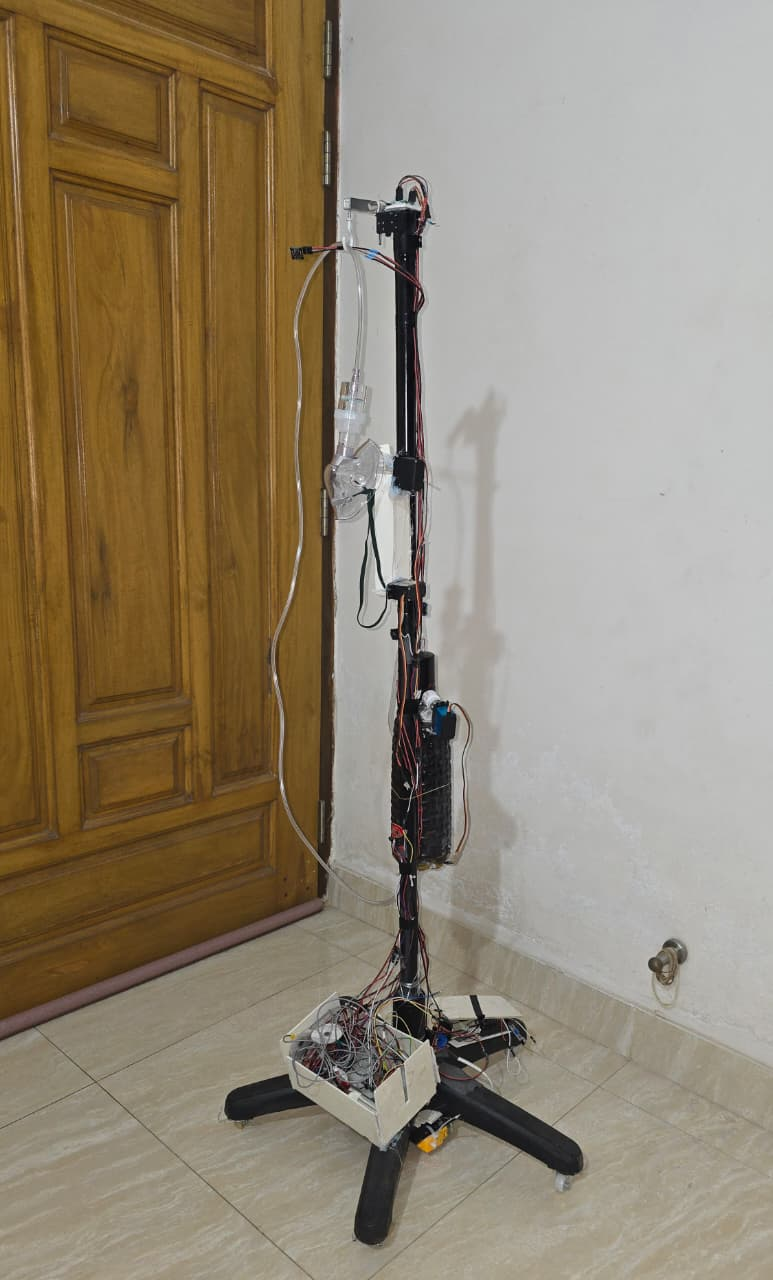
\includegraphics[width=\linewidth]{6.jpeg}};
\begin{scope}[x={(pic.south east)},y={(pic.north west)}]
\tikzset{partmarker/.style={circle,draw=black,fill=white,inner sep=2pt,font=\fontsize{8}{9}\selectfont},pointer/.style={-{Latex[length=1.5mm]},thick,preaction={draw=white,line width=2pt}}}
\node[partmarker] (a) at (0.78,0.84) {1};\draw[pointer] (a) -- (0.49,0.83);
\node[partmarker] (b) at (0.79,0.60) {2};\draw[pointer] (b) -- (0.47,0.62);
\node[partmarker] (c) at (0.79,0.38) {3};\draw[pointer] (c) -- (0.55,0.41);
\node[partmarker] (d) at (0.17,0.18) {4};\draw[pointer] (d) -- (0.46,0.17);
\node[partmarker] (e) at (0.79,0.06) {5};\draw[pointer] (e) -- (0.67,0.09);
\end{scope}
\end{tikzpicture}
\par\smallskip\footnotesize (a) Overall prototype. 1: load-cell/hook; 2: mask/tubing; 3: mounted actuation assembly; 4: electronics enclosure; 5: caster base.
\end{minipage}\hfill
\begin{minipage}[t]{0.31\textwidth}
\centering
\begin{tikzpicture}
\node[anchor=south west,inner sep=0] (pic) at (0,0) {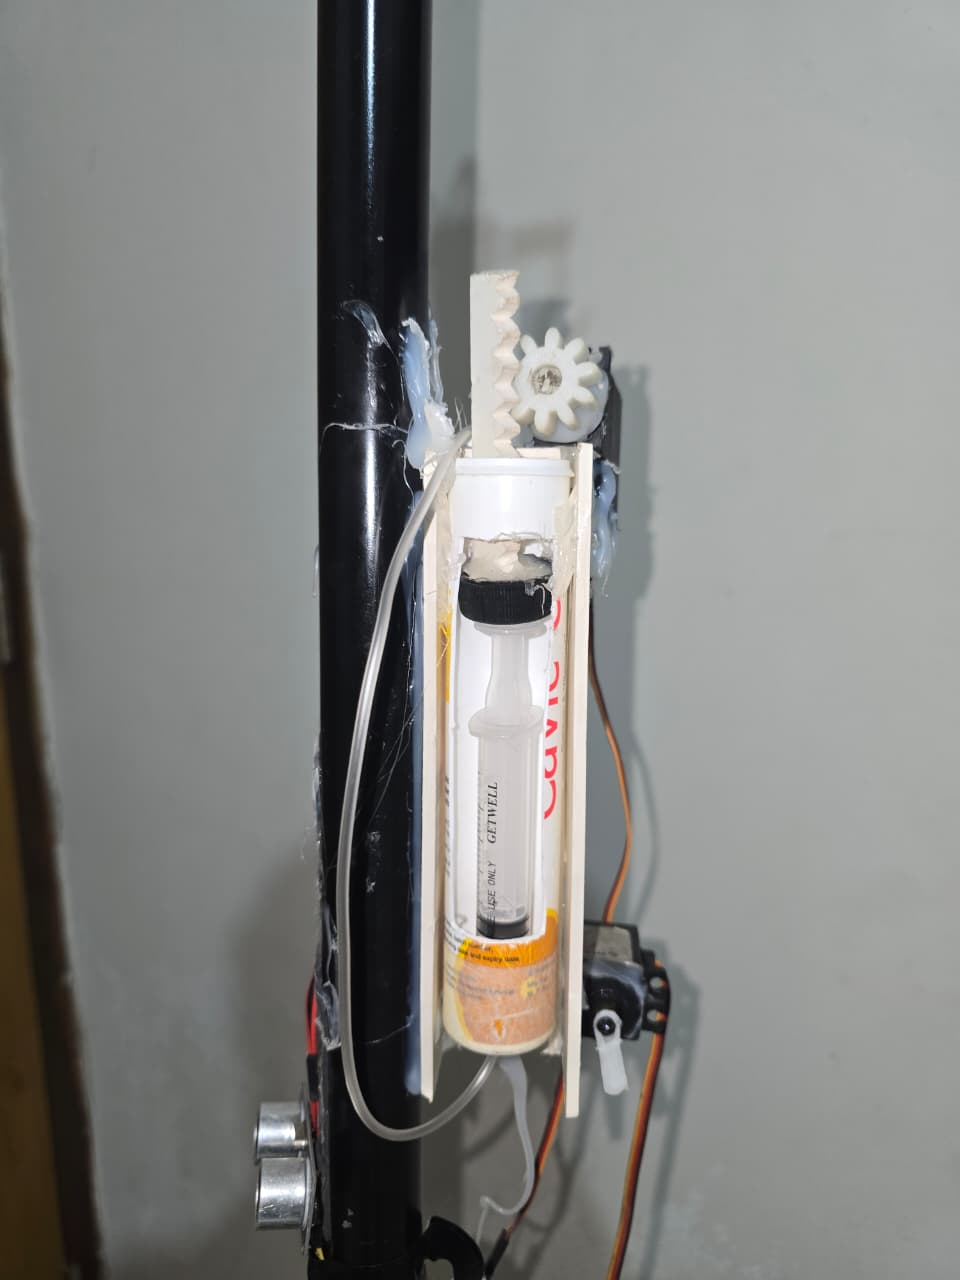
\includegraphics[width=\linewidth]{3.jpeg}};
\begin{scope}[x={(pic.south east)},y={(pic.north west)}]
\tikzset{partmarker/.style={circle,draw=black,fill=white,inner sep=2pt,font=\fontsize{8}{9}\selectfont},pointer/.style={-{Latex[length=1.5mm]},thick,preaction={draw=white,line width=2pt}}}
\node[partmarker] (a) at (0.80,0.73) {1};\draw[pointer] (a) -- (0.58,0.71);
\node[partmarker] (b) at (0.83,0.44) {2};\draw[pointer] (b) -- (0.55,0.47);
\node[partmarker] (c) at (0.88,0.19) {3};\draw[pointer] (c) -- (0.65,0.22);
\end{scope}
\end{tikzpicture}
\par\smallskip\footnotesize (b) Syringe construction. 1: rack and gear; 2: syringe/guide; 3: visible servo attachment. Photographs do not quantify delivered dose.
\end{minipage}\hfill
\begin{minipage}[t]{0.31\textwidth}
\centering
\begin{tikzpicture}
\node[anchor=south west,inner sep=0] (pic) at (0,0) {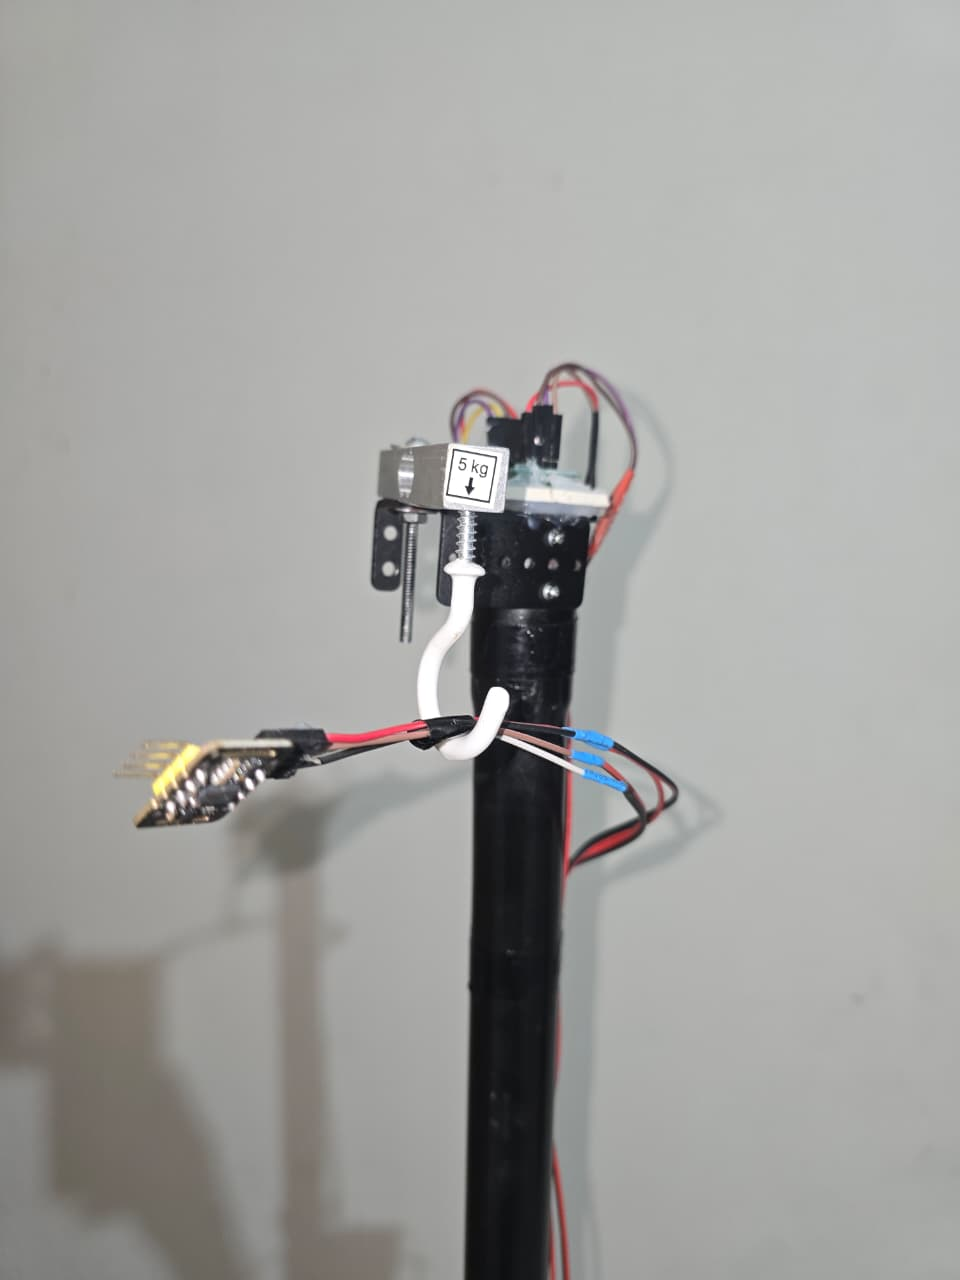
\includegraphics[width=\linewidth]{4.jpeg}};
\begin{scope}[x={(pic.south east)},y={(pic.north west)}]
\tikzset{partmarker/.style={circle,draw=black,fill=white,inner sep=2pt,font=\fontsize{8}{9}\selectfont},pointer/.style={-{Latex[length=1.5mm]},thick,preaction={draw=white,line width=2pt}}}
\node[partmarker] (a) at (0.23,0.66) {1};\draw[pointer] (a) -- (0.48,0.63);
\node[partmarker] (b) at (0.79,0.48) {2};\draw[pointer] (b) -- (0.49,0.46);
\node[partmarker] (c) at (0.82,0.75) {3};\draw[pointer] (c) -- (0.62,0.65);
\end{scope}
\end{tikzpicture}
\par\smallskip\footnotesize (c) Load sensing mount. 1: load cell labeled 5~kg; 2: hanging hook; 3: wiring and support electronics.
\end{minipage}
\caption{Annotated photographs supplied with the project: overall view (photograph~6), syringe assembly (photograph~3), and load-cell mount (photograph~4). Numbered callouts identify visible parts without assigning unreadable model labels.}\label{fig:prototypephotos}
\end{figure*}

\begin{figure}[!t]
\centering
\begin{tikzpicture}
\node[anchor=south west,inner sep=0] (pic) at (0,0) {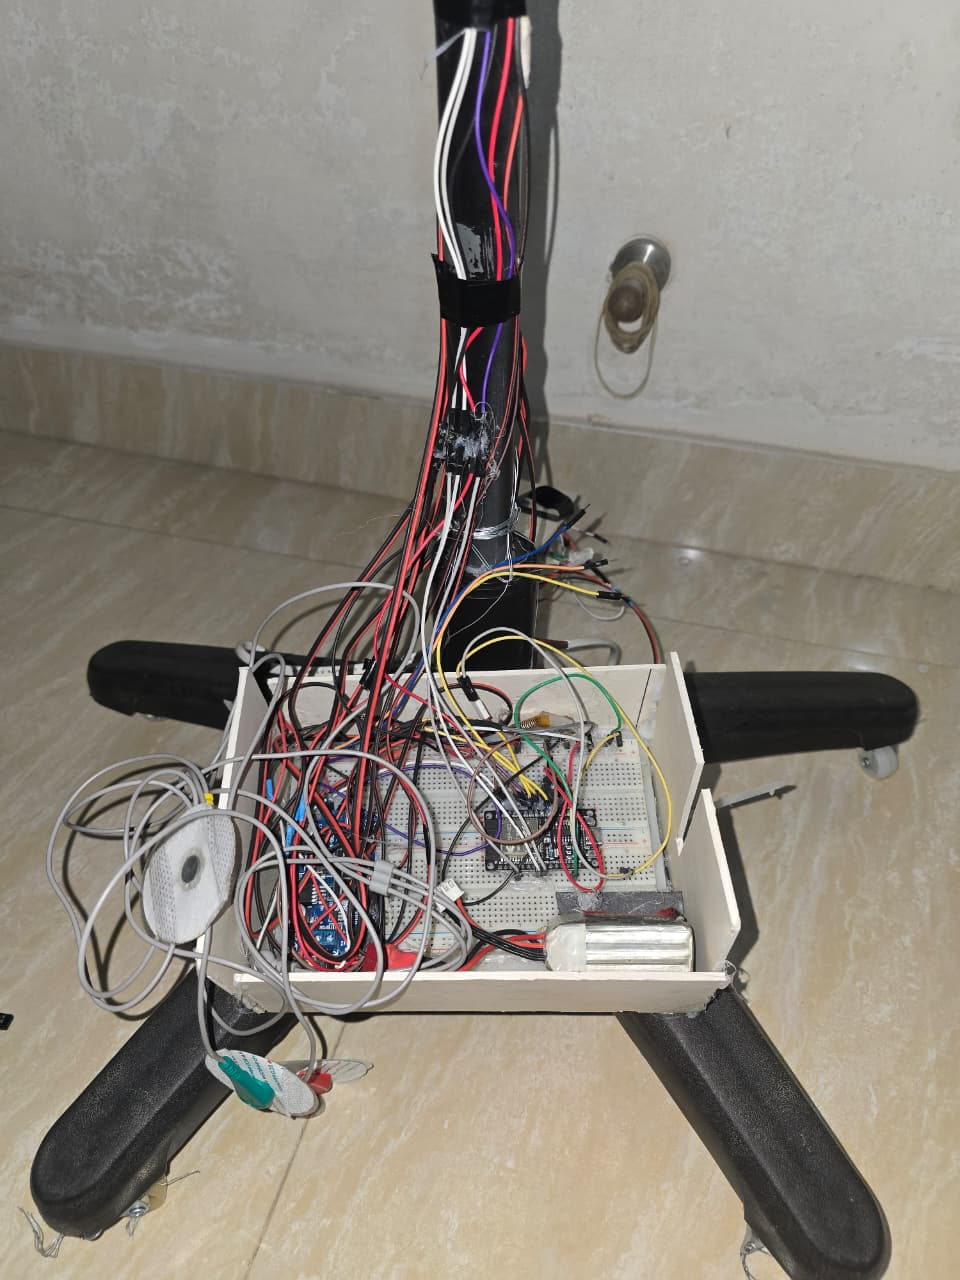
\includegraphics[width=0.83\columnwidth]{1.jpeg}};
\begin{scope}[x={(pic.south east)},y={(pic.north west)}]
\tikzset{partmarker/.style={circle,draw=black,fill=white,inner sep=2pt,font=\fontsize{8}{9}\selectfont},pointer/.style={-{Latex[length=1.5mm]},thick,preaction={draw=white,line width=2pt}}}
\node[partmarker] (a) at (0.86,0.44) {1};\draw[pointer] (a) -- (0.56,0.36);
\node[partmarker] (b) at (0.82,0.19) {2};\draw[pointer] (b) -- (0.66,0.30);
\node[partmarker] (c) at (0.13,0.16) {3};\draw[pointer] (c) -- (0.26,0.16);
\end{scope}
\end{tikzpicture}
\caption{Base electronics in photograph~1. 1: controller-board area; 2: breadboard wiring; 3: electrode pads/cables. Wiring obscures some labels, so exact component identities are taken from the source/wiring inventory rather than inferred from this view.}\label{fig:electronics}
\end{figure}



\section{Results}\label{sec:results}
\subsection{Available Evidence and Evaluation Method}
The available evidence comprises the assembled-system photographs, the implementation source, and saved website/database screenshots. The slides provide objectives and feature descriptions, but no tabulated trials, reference measurements, instrument readings, timestamps, or experimental logs. The results below therefore report directly visible states and source-derived behavior separately. Numerical accuracy, dose error, and actual latency cannot be calculated from the archive.

\subsection{Captured Dashboard and Database State}
Fig.~\ref{fig:doctorresult} shows the doctor interface with a remaining-fluid estimate of 324.1~mL, a saline stop setting of 320~mL, an \emph{Open} valve state, and a \emph{Standby} syringe state. The supplied Firebase console capture shows the same \code{current_ml}, threshold, and status values. This agreement supports consistency between the captured dashboard and stored data at that observation; it does not establish the correctness of the load-cell calibration or prove a complete actuation sequence.

The state also agrees with the code's strict remaining-volume rule. Since $324.1<320$ is false, (\ref{eq:saline}) does not request closure. This interpretation is important because the threshold is a remaining-volume cutoff, rather than a target volume already delivered. Screenshots~6 and 7 duplicate screenshots~1 and 2 respectively and are not counted as additional trials.

\begin{figure*}[!t]
\centering
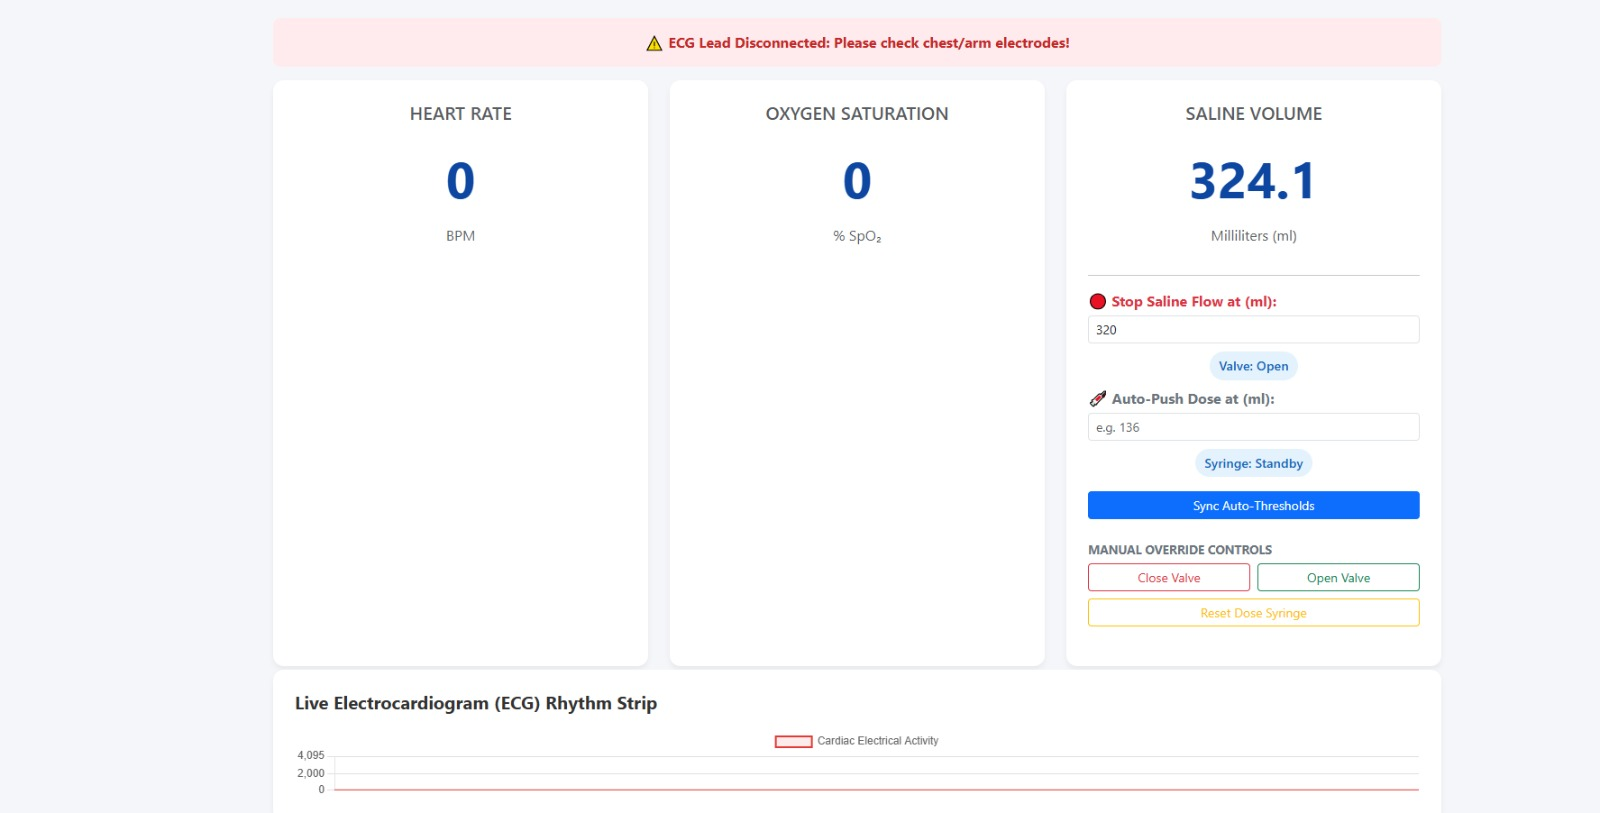
\includegraphics[width=0.97\textwidth]{web_1.jpeg}
\caption{Supplied doctor dashboard capture: estimated fluid 324.1~mL, configured stop threshold 320~mL, valve Open, syringe Standby, and unavailable physiological values. The zero ECG trace and disconnection banner document an interface state, without establishing a valid measured rhythm.}\label{fig:doctorresult}
\end{figure*}

Table~\ref{tab:observed} records the observation without assigning unmeasured performance values. The additional \code{saline_ml} and \code{saline_threshold} entries visible in the console screenshot are not read or written by the current active dashboard/firmware paths, and are not treated as the implemented data contract.

\begin{table}[!t]
\caption{Values Visible in the Supplied Captures}\label{tab:observed}
\centering\footnotesize
\begin{tabularx}{\columnwidth}{@{}P{0.31\columnwidth}P{0.20\columnwidth}Y@{}}
\toprule
Quantity & Visible value & Supported interpretation \\
\midrule
Fluid estimate & 324.1~mL & Displayed estimate; calibration unverified. \\
Saline stop setting & 320~mL & Positive remaining-volume cutoff. \\
Saline state & Open & Consistent with estimate above cutoff. \\
Dose trigger & 0 & Volume-trigger rule disabled in console snapshot. \\
Syringe state & Standby & No stroke shown at capture time. \\
Pulse / oxygen & 0 / 0 & Unavailable readings; no physiological accuracy evidence. \\
ECG & 0 & Doctor view shows disconnection warning and zero plot. \\
\bottomrule
\end{tabularx}
\end{table}

\subsection{Patient and Family Interface Outputs}
Fig.~\ref{fig:patientresult} shows the patient dashboard labeling the zero pulse and oxygen values as \emph{Sensor Ready / Place Finger}. Fig.~\ref{fig:familyresult} shows the corresponding family view. The family implementation excludes zero values from its positive-low-reading tests, so the lack of a family alarm in this capture is consistent with its code. It does not demonstrate that an abnormal valid measurement was detected or that a notification reached a caregiver.

\begin{figure}[!t]
\centering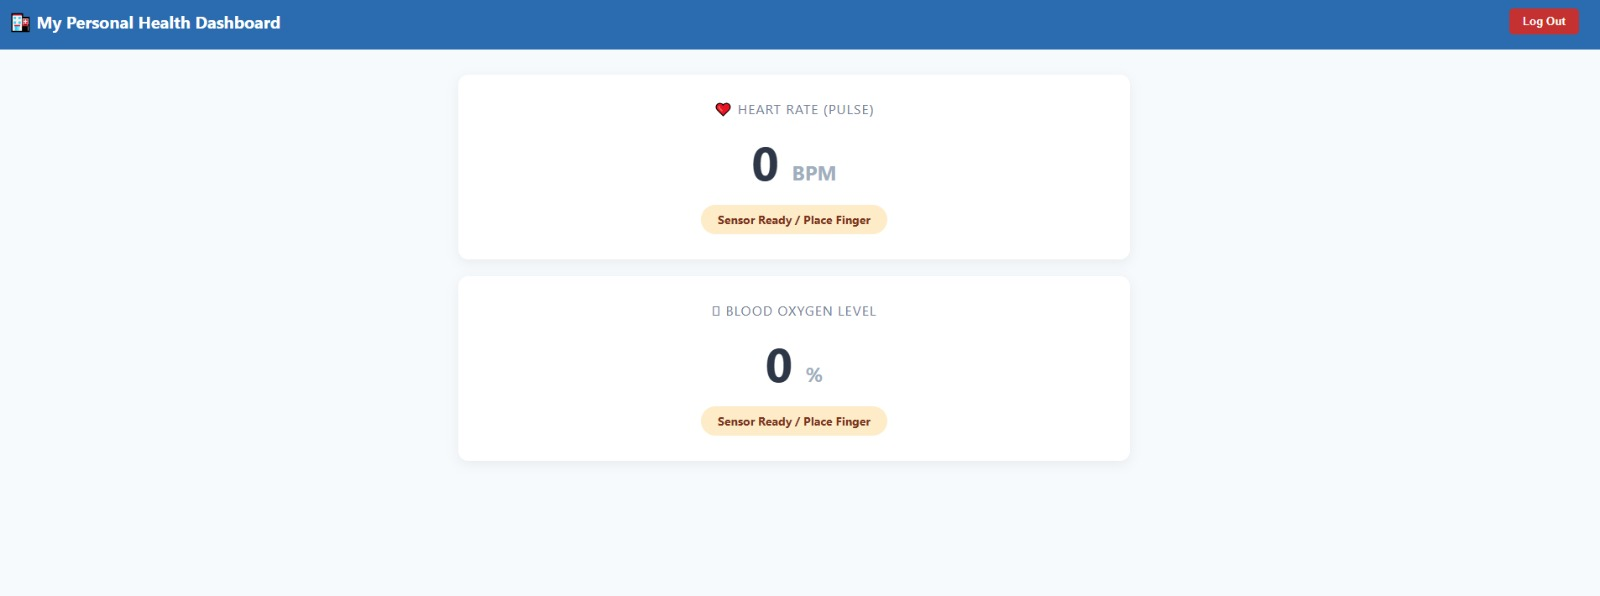
\includegraphics[width=\columnwidth]{web_5.jpeg}
\caption{Patient dashboard capture displaying zero readings and sensor-ready messages. The image demonstrates the unavailable-reading presentation rather than validated physiological sensing.}\label{fig:patientresult}
\end{figure}
\begin{figure}[!t]
\centering
\includegraphics[width=\columnwidth]{web_2.jpeg}
\caption{Family/guardian dashboard capture. No alert is visible for the captured zero values, which the implemented alert condition excludes.}\label{fig:familyresult}
\end{figure}

The account-creation screenshot contains the patient, family/guardian, and medical-doctor role choices. Source inspection confirms the intended authentication and routing sequence. Successful registration of every role, enforcement of doctor privileges, and protected access to telemetry are not established by that single screenshot.

\subsection{Source-Derived Output Conditions}
The prototype's key output conditions are explicit in the firmware. The following excerpt is taken from the control-condition portion of \code{main.c}; it contains no credentials:
\begin{quote}\footnotesize
\begin{verbatim}
bool saline_stop_active =
  (saline_stop_ml > 0 &&
   current_ml < saline_stop_ml);
bool weight_trigger =
  (dose_trigger_ml > 0 &&
   current_ml < dose_trigger_ml);
bool o2_emergency =
  (smooth_spo2 > 0 &&
   smooth_spo2 < OXYGEN_DANGER_LEVEL);
\end{verbatim}
\end{quote}
When \code{o2_emergency} is true, the output branch calls \code{gpio_set_level(BUZZER_PIN, 1)} and advances the oxygen-designated servo angle. The code therefore establishes the command path from an estimated sensor value to a GPIO/PWM output. The supplied photographs do not capture the buzzer energized or provide measured oxygen flow, so physical alarm activation and treatment delivery are not reported as observed results.

Table~\ref{tab:logiccases} presents illustrative boundary cases derived from these conditions. These are analytic examples, not newly conducted bench tests or recorded patient data.
\begin{table*}[!t]
\caption{Illustrative Input-to-Output Cases Derived from the Firmware}\label{tab:logiccases}
\centering\small
\begin{tabularx}{\textwidth}{@{}P{0.21\textwidth}P{0.27\textwidth}YY@{}}
\toprule
Case & Assumed inputs & Programmed outcome & Evidence status \\
\midrule
Captured saline state & $V=324.1$~mL, $T_s=320$~mL & Closing condition false; target moves toward open. & Values/status visible in saved captures and consistent with code. \\
Saline threshold equality & $V=320$~mL, $T_s=320$~mL & Strict comparison false; does not begin closing. & Boundary example from source only. \\
Below saline cutoff & $V=319$~mL, $T_s=320$~mL & Servo moves toward clamp; Closing then Stopped if condition persists. & Source-derived case; no matching observed sequence supplied. \\
Volume-triggered syringe & $V=135$~mL, $T_d=136$~mL; cycle inactive & Begins fixed forward/return angle sequence. & Source-derived case; delivered volume unmeasured. \\
Low estimated oxygen & $S=84\%$ with usable optical input & Buzzer GPIO high; oxygen-designated servo advances. & Source-derived case; alarm/flow not experimentally documented. \\
Unavailable optical input & Infrared count below 20000 & Pulse and oxygen estimates zero; positive-low-oxygen condition false. & Source branch; zero outputs are visible, but raw optical input was not recorded. \\
ECG lead off & LO+ or LO$-$ high & ECG value forced to zero; doctor page shows warning. & Source branch; warning visible, input-pin state unrecorded. \\
\bottomrule
\end{tabularx}
\end{table*}

\subsection{Timing and Efficiency That Can Be Inferred}
The 20~ms programmed loop delay and angular increments yield nominal delay-only travel times: $90\times20$~ms $=1.8$~s for a $180^{\circ}$ saline/oxygen command, $180\times20$~ms $=3.6$~s for the syringe's forward stroke, and about 1.8~s for its return. Sensor access and transition iterations add time, and mechanical motion may differ from the command sequence. These values are calculations from the implementation, not measured response times.

The cloud task delays two seconds after completing its requests, so it offers periodic latest-value publication with additional HTTP overhead. The doctor plot appends one ECG value per database callback rather than a timestamped waveform packet. Consequently, the captured flat plot and software timing do not establish ECG waveform fidelity. No current measurements, battery-capacity specification, deployment uptime, or itemized purchase costs are provided, so energy efficiency, battery life, and total cost remain unquantified.

\subsection{Experimental Validation Required for Performance Claims}
Table~\ref{tab:validation} specifies the missing measurements and an appropriate way to obtain them. These procedures are proposed future evaluation, not completed experiments. Fluid and syringe trials should use a laboratory collection setup; any human physiological study requires the relevant supervision and consent arrangements.

\begin{table*}[!t]
\caption{Proposed Validation Plan; No Results Are Claimed for These Tests}\label{tab:validation}
\centering\small
\begin{tabularx}{\textwidth}{@{}P{0.20\textwidth}YY@{}}
\toprule
Subsystem & Proposed procedure & Record and evaluation metric \\
\midrule
Fluid estimate & Tare the empty assembly; apply known loads/volumes across its range; repeat static and disturbed trials. & Reference/estimated volume pairs; mean absolute error, maximum error, repeatability, and mounting conditions. \\
Saline stopping & Move the measured estimate through positive thresholds, equality, and disabled settings; collect remaining leakage after closure. & Input, GPIO/PWM time, physical closure time, state sequence, and residual fluid movement. \\
Syringe mechanism & Calibrate syringe geometry/travel using collected fluid; repeat full-stroke trials under specified loads. & Reference delivered volume, variation, backlash, stalls, and mechanical limits. \\
Pulse / SpO\textsubscript{2} & Compare synchronized valid outputs with an appropriate reference instrument and document signal/motion conditions. & Paired readings, acquisition availability, agreement errors, and recovery after signal loss. \\
ECG channel & Use a known simulator/reference signal and record locally timestamped samples; exercise both lead-off inputs. & Sampling interval/jitter, signal agreement, lead-off detection, and cloud information loss. \\
Cloud/control & Timestamp a setting change, device receipt, output command, and browser status; repeat with delays/disconnection. & Median/maximum end-to-end times, failed writes, stale-data behavior, and recovery. \\
Power and operation & Measure voltage/current with Wi-Fi and servos active, and observe resets/stalls on the actual supply. & Peak current, energy per interval, operating duration, and brownout behavior. \\
\bottomrule
\end{tabularx}
\end{table*}

For $N$ paired reference and estimated volumes, a reproducible accuracy summary would include
\begin{equation}
\mathrm{MAE}_V=\frac{1}{N}\sum_{i=1}^{N}|\hat V_i-V_i^{\mathrm{ref}}|\quad(\mathrm{mL}).
\end{equation}
An end-to-end control measurement would separately record database write time, device receipt time, and physical actuator response. No values for these metrics are inserted because the required paired records and timestamps are absent.


\section{Discussion}\label{sec:discussion}
\subsection{Limitations and Examples of Unexpected Operation}
\subsubsection{Calibration and Unobserved Delivery}
The current fluid conversion has a fixed offset/divisor and no supplied calibration, tare, or density record. Moving the stand, changing the supported container, or changing mechanical loading can therefore produce an unreliable remaining-volume estimate. The syringe and oxygen-designated mechanisms receive angle commands without delivered-volume, pressure, flow, or external position feedback. A displayed \emph{Stopped} or \emph{Pushed} state represents the firmware's sequence state and may not match physical delivery if a linkage slips or a servo stalls.

\subsubsection{Repeated Dose Scheduling and Reset Semantics}
A configured time trigger remains true throughout its matching minute. Once the syringe completes its forward/return cycle, the same condition can start another cycle; no executed-event identifier or date latch prevents repetition. Clearing the browser's dose threshold also does not abort an active cycle or clear a previously parsed time schedule. These are concrete examples in which user expectations and the programmed behavior may differ, and require an explicit once-per-event schedule and cancel/acknowledgment mechanism before a dosing claim is justified.

\subsubsection{Signal Availability and Alarm Meaning}
The pulse buffer accepts only values strictly between 50 and 130~BPM; a signal outside that range can be rejected while the display retains prior buffered values. SpO\textsubscript{2} is restricted to 80--100\%, so the interface cannot display lower estimates. Finger-signal loss sets the oxygen estimate to zero and disables the positive-low-oxygen alarm condition, making sensor unavailability distinct from an emergency reading. These behaviors need explicit signal-validity/freshness reporting rather than interpretation as a complete physiological alarm system.

The family view's low-pulse alarm requires a positive BPM below 50, while the firmware normally admits pulse estimates above 50. That combination limits the usefulness of the family low-pulse branch for this telemetry source. The patient view labels both low and high nonzero out-of-range pulse readings as \emph{Elevated Heart Rate}, and the doctor page equates ECG zero with disconnected leads. The interfaces need consistent thresholds and separate validity fields to avoid misleading labels.

\subsubsection{Network, Security, and Reproducibility}
Telemetry has no timestamp, sequence number, stale-data indication, or device identifier. During a connectivity failure, the browser may retain old values and the firmware may continue with previous settings. The HTTP code performs limited status/error validation and uses text searches instead of a structured JSON parser; network and control tasks also share state without an atomic snapshot. These limitations affect command reliability and interpretation of the displayed values.

The archived configuration explicitly disables TLS server verification, and credentials are embedded in the source. The doctor page lacks an authentication guard, registration permits self-selection of the doctor role, and no database-rule file establishes the deployed authorization policy. Server-enforced access rules, authenticated device requests, certificate verification, command validation, and restricted telemetry access are required improvements~\cite{firebaserules,idfhttp}. The shared database paths and flash-size/toolchain inconsistencies further limit reproducibility and extension to multiple patients.

\subsection{Depth of Knowledge (P1)}
The project requires knowledge across microcontroller architecture, ADC and serial interfaces, PWM timing, filtering, FreeRTOS tasks, network protocols, cloud data, and electromechanical design. It also requires understanding why a sensor output, a filtered estimate, a software actuator state, and an independently measured delivered quantity are different forms of evidence. These interacting domains support the depth-of-knowledge mapping for P1.

\subsection{Conflicting Requirements and Trade-offs (P2)}
Affordability and a single-controller design favor inexpensive sensors and servo mechanisms, while accurate delivery and robust monitoring require calibration, feedback, and additional fault detection. Strong smoothing improves display stability but delays changes; separating cloud requests from the local loop improves continuity but introduces shared-state synchronization requirements. The implementation therefore trades hardware simplicity and development effort against measurement fidelity, response predictability, and verified control.

\subsection{Two Alternative Designs and Analysis (P3)}
\subsubsection{Alternative 1: Instrumented Stepper/Lead-Screw Syringe}
A stepper motor, lead screw, homing switches, and plunger-position/force sensing would make commanded displacement more explicit than a fixed servo sweep. With a measured syringe bore area $A$ and plunger displacement $\Delta x$, the nominal geometric delivery is $\Delta V=A\Delta x$, but backlash, fluid compliance, and pressure still require collection-based calibration. This alternative adds motor-driver, mechanical, and sensing cost, yet offers a clearer route to volume/rate control and fault detection than the archived mechanism.

\subsubsection{Alternative 2: Passive Monitor with Manual Infusion Control}
A monitoring-only device could combine load-cell and optical drop sensing, retain the physiological channels, and alert a caregiver without remotely actuating fluid delivery. This would reduce actuator complexity and associated command hazards, while still requiring reliable calibration and alarm evaluation. It would provide less automation and retain manual response time, but could be a more focused first stage for validating sensing and caregiver usability. The optical/load-cell integration in prior work~\cite{lee2021} provides a relevant design precedent.

\subsection{Impact and Familiarity of Issues (P4)}
The intended application extends beyond routine computer-science coursework into medical workflow, fluid mechanics, physiological measurement, and human interaction. The potential benefit is a common view of fluid estimates and sensor status that can support caregiver attention, particularly where equipment cost matters. That benefit remains an engineering objective; there is no supplied evidence of improved clinical outcomes or reduced staff workload, and those questions require domain expertise and evaluation with intended users.

\subsection{Standards, Manuals, and Ethical Considerations (P5)}
Relevant references include device documentation, the NXP I\textsuperscript{2}C specification, and ESP-IDF/Firebase manuals, although the archive contains neither electrical/timing compliance measurements nor a record of the manuals originally studied by the team~\cite{max30102,ad8232,i2cmanual,idfhttp,firebaserules}. The 100~kHz I\textsuperscript{2}C setting matches Standard-mode, while disabled TLS verification departs from authenticated server verification; use of a named protocol alone therefore does not establish complete compliance. The ACM code motivates honest performance claims, privacy, and avoidance of harm~\cite{acmethics}, while FDA infusion guidance provides a comparator for hazard analysis, alarm behavior, and evaluation~\cite{fdaguidance}, without establishing certification of this prototype or compliance with local clinical requirements.

\subsection{Stakeholders and Requirement Incorporation (P6)}
The implemented views identify doctors, patients, and family/guardians as intended stakeholders, and the slides also identify nursing workload as a motivation. Their represented requirements differ: clinicians need telemetry and controllable thresholds, patients need a simple display, and families need accessible status and warnings. However, no interview notes, stakeholder approvals, funding discussions, or usability-study results were supplied. P6 is therefore left unmarked until actual consultation and resulting design changes are documented; intended users alone do not demonstrate stakeholder involvement.

\subsection{Module Interdependence (P7)}
Sensor interfaces, local control, cloud synchronization, and browser views form recognizable modules, and the local loop can continue while the network task is delayed. Nevertheless, remote controls depend on Wi-Fi/Firebase and a shared settings schema, while browser status depends on device publication and both tasks share mutable variables. The physical sensors/actuators are coupled to firmware pins and calibration, so modular files and separate tasks provide partial separation rather than complete independence.

\subsection{Complex Engineering Problem Mapping}
Table~\ref{tab:cep} marks the aspects discussed with evidence or design analysis. P5 represents the documented interface/security/ethical considerations, not a certification claim. P6 remains pending because consultation evidence is absent.
\begin{table}[!t]
\caption{Complex Engineering Problem Mapping}\label{tab:cep}
\centering\small
\begin{tabular}{ccccccc}
\toprule
P1 & P2 & P3 & P4 & P5 & P6 & P7 \\
\midrule
$\checkmark$ & $\checkmark$ & $\checkmark$ & $\checkmark$ & $\checkmark$ & --- & $\checkmark$ \\
\bottomrule
\end{tabular}
\par\smallskip\footnotesize
P1: depth of knowledge; P2: conflicting requirements; P3: depth of analysis; P4: familiarity of issues; P5: extent of applicable codes; P6: extent of stakeholders; P7: interdependence.
\end{table}

\section{Conclusion}\label{sec:conclusion}
MediSmart integrates an ESP32, optical and ECG sensing, a load-cell fluid estimate, three servo-control channels, and a local buzzer with Firebase-based doctor, patient, and family interfaces. The archived implementation provides remaining-volume threshold control and a syringe motion sequence, with a captured 324.1~mL dashboard estimate and an open-valve state consistent with the configured 320~mL cutoff.

Separate local and network tasks support continued control processing during HTTP requests, but measured latency, accuracy, dose delivery, cost, and power efficiency are not established by the supplied evidence. Future development should prioritize fluid and syringe calibration, independently observed actuator/flow states, once-per-event scheduling, and explicit signal-validity reporting. Timestamped waveform acquisition, consistent alert policies, authenticated access, verified TLS, and device-specific data paths would strengthen monitoring reliability and extend the architecture. Controlled bench evaluation and documented stakeholder feedback should precede any claim of clinical benefit; the project repository link is included in the references, while the demonstration-video link awaits completion~\cite{projectgithub,projectyoutube}.


\section*{Acknowledgment}
\ProjectAcknowledgment

\begin{thebibliography}{99}
\bibitem{lee2021}
J.-K. Lee, K.-C. Yoon, and K. G. Kim, ``Design of a remote monitoring system based on optical sensors to prevent medical accidents during fluid treatment,'' \emph{Applied Sciences}, vol.~11, no.~21, Art.~10124, 2021, doi:~10.3390/app112110124. [Online]. Available: \url{https://www.mdpi.com/2076-3417/11/21/10124}.

\bibitem{contardi2022}
U. A. Contardi, M. Morikawa, B. Brunelli, and D. V. Thomaz, ``MAX30102 photometric biosensor coupled to ESP32-webserver capabilities for continuous point of care oxygen saturation and heartrate monitoring,'' \emph{Engineering Proceedings}, vol.~16, no.~1, Art.~9, 2022, doi:~10.3390/IECB2022-11114. [Online]. Available: \url{https://www.mdpi.com/2673-4591/16/1/9}.

\bibitem{kok2024}
C. L. Kok, C. K. Ho, T. K. Lee, Z. Y. Loo, Y. Y. Koh, and J. P. Chai, ``A novel and low-cost cloud-enabled IoT integration for sustainable remote intravenous therapy management,'' \emph{Electronics}, vol.~13, no.~10, Art.~1801, 2024, doi:~10.3390/electronics13101801. [Online]. Available: \url{https://www.mdpi.com/2079-9292/13/10/1801}.

\bibitem{max30102}
Analog Devices / Maxim Integrated, ``MAX30102: High-sensitivity pulse oximeter and heart-rate sensor for wearable health,'' data sheet, Rev.~1, Oct.~2018. [Online]. Available: \url{https://www.analog.com/media/en/technical-documentation/data-sheets/max30102.pdf}. Accessed: Oct.~8, 2026.

\bibitem{ad8232}
Analog Devices, ``AD8232: Single-lead, heart rate monitor front end,'' data sheet, Rev.~D. [Online]. Available: \url{https://www.analog.com/media/en/technical-documentation/data-sheets/ad8232.pdf}. Accessed: Oct.~8, 2026.

\bibitem{firebaserules}
Google Firebase, ``Understand Firebase Realtime Database Security Rules.'' [Online]. Available: \url{https://firebase.google.com/docs/database/security}. Accessed: Oct.~8, 2026.

\bibitem{i2cmanual}
NXP Semiconductors, ``I\textsuperscript{2}C-bus specification and user manual,'' UM10204, Rev.~7.0, Oct.~1, 2021. [Online]. Available: \url{https://www.nxp.com/docs/en/user-guide/UM10204.pdf}.

\bibitem{idfhttp}
Espressif Systems, ``ESP HTTP Client,'' \emph{ESP-IDF Programming Guide}. [Online]. Available: \url{https://docs.espressif.com/projects/esp-idf/en/stable/esp32/api-reference/protocols/esp_http_client.html}. Accessed: Oct.~8, 2026.

\bibitem{acmethics}
Association for Computing Machinery, ``ACM Code of Ethics and Professional Conduct,'' Jun.~22, 2018. [Online]. Available: \url{https://www.acm.org/code-of-ethics}.

\bibitem{fdaguidance}
U.S. Food and Drug Administration, ``Infusion pumps total product life cycle: Guidance for industry and FDA staff,'' Dec.~2, 2014. [Online]. Available: \url{https://www.fda.gov/media/78369/download}.

\bibitem{projectgithub}
MediSmart project team, ``Project source-code repository.'' \ProjectGithub.

\bibitem{projectyoutube}
MediSmart project team, ``Project demonstration video.'' \ProjectYoutube.
\end{thebibliography}

\appendices
\section{Setup and Laboratory Operating Instructions}
\label{app:operating-instructions}

These instructions support supervised, nonclinical bench demonstrations. Use water and mechanical mock loads; keep the infusion, syringe, and oxygen-designated mechanisms disconnected from patients. Verify wiring, mechanical clearance, supply capacity, and a means of removing actuator power before starting. The supplied photographs and wiring sketches do not establish clinical or electrical safety.

\subsection{Firmware Preparation}
Install VS Code with PlatformIO IDE and the board's USB serial driver, then open \path{medismart/medismartVscode/} as the PlatformIO project. Select environment \code{esp32dev}, board \code{esp32dev}, and framework \code{espidf}; the application is ESP-IDF C. Regenerate the included editor/debug configuration because its absolute paths belong to another workstation. Record the installed toolchain and framework versions when reproducing the build.

In \path{src/main.c}, replace the Wi-Fi settings with \placeholder{LAB SSID} and \placeholder{LAB PASSWORD}, and configure matching settings/vitals endpoints for \placeholder{LAB FIREBASE DATABASE URL}. Keep credential values out of submitted listings. Confirm the physical flash capacity: \code{platformio.ini} requests 4~MB, whereas \code{sdkconfig.esp32dev} selects 2~MB. Reconcile the saved configuration and board settings before uploading. The following commands run from the firmware project directory:
\begin{quote}
\small
\code{pio run -e esp32dev}\\
\code{pio run -e esp32dev -t upload}\\
\code{pio device monitor -b 115200}
\end{quote}
Select the correct serial port if automatic detection fails. Inspect build/upload output and the serial dashboard; a successful compilation alone does not verify connected sensors or mechanisms.

\subsection{Cloud and Browser Configuration}
Use an isolated laboratory database. Configure Firebase Realtime Database and email/password Authentication, then make the browser pages and firmware reference the same project. Replace the doctor page's API-key, sender-ID, and application-ID placeholders with that project's web configuration. The supplied \code{firebase.json} specifies static content in \path{medismart/public/}; it supplies no database rules.

Before protected operation, implement server-side rules that restrict telemetry writes to the device and settings changes to approved operators. Registration-selected roles must not authorize themselves. This requires corresponding firmware REST authentication and authentication/role checks in the doctor page, which are absent from the supplied code. Restore TLS server verification before protected deployment. Official rule and REST-authentication guidance is available at \url{https://firebase.google.com/docs/database/security} and \url{https://firebase.google.com/docs/database/rest/auth}; secure operation cannot be achieved by changing browser navigation alone.

Open \code{login.html} explicitly: the supplied root page remains Firebase's welcome template. Register a laboratory account using the patient, family, or doctor selection, then sign in. Login reads the saved role and redirects accordingly. Patient/family pages display the shared vital stream; the doctor page adds fluid estimates, statuses, settings, and a rolling received-value ECG plot. These screens provide navigation rather than verified role-based authorization in the current implementation.

\subsection{Startup and Controls}
After power-up, verify Wi-Fi, database updates, sensor contact, and known-weight/volume calibration before interpreting readings. SNTP uses \code{pool.ntp.org}; the POSIX timezone \code{UTC-6} represents Dhaka's UTC+06:00. Confirm actual synchronization separately because startup does not wait for valid time. Record local/remote observation times to identify stale telemetry.

\emph{Sync Auto-Thresholds} writes both remaining-volume thresholds. A positive saline threshold closes its valve only when the estimate is strictly lower; equality does not trigger closure. A positive dose threshold starts a fixed syringe stroke under the same comparison and does not specify delivered drug volume. Blank or invalid inputs become zero, disabling the corresponding volume condition.

\emph{Open Valve} writes a zero saline threshold. \emph{Close Valve} writes 9999, producing a closure condition only while the estimate is below that sentinel. \emph{Reset Dose Syringe} clears the dose-volume threshold; it does not cancel an active stroke or immediately retract the syringe. Check subsequent physical movement and telemetry because buttons provide no execution acknowledgement.

The firmware parses \code{dose_time}, but the supplied dashboard has no schedule editor. Its matching-minute condition can repeat cycles without an execution latch; leave scheduling disabled until this behavior is corrected and tested. Supervise every bench cycle, record sensor-invalid/network-loss cases, and remove actuator power for a physical stop. Dashboard zeros, software angles, and status labels do not prove physiological validity or delivered volume.

% Begin the artifact inventory in the next column to balance the final page.
\newpage
\section{Project Artifact Traceability}
\label{app:artifact-traceability}

The report uses the following supplied artifact groups; generated build files are not experimental evidence:
\begin{itemize}
\item \path{Project_slides/}: the project presentation establishes its title, team, and concept; slide-only features require implementation evidence.
\item \path{Project_images/1.jpeg} through \code{6.jpeg}: assembly, mechanisms, sensors, and electronics photographs.
\item \path{Website_images/web_1.jpeg} through \code{web_7.jpeg}: dashboard, registration, and database captures; two pairs repeat the same screens.
\item \path{medismart/}: sensor and actuator wiring PNGs, \code{firebase.json}, \path{public/} browser sources, and \path{medismartVscode/} firmware/build configuration.
\item \path{CSE_4326_Project_Paper/}: the IEEE master, chapter files, metadata placeholders, \code{IEEEtran.cls}, \code{IEEEtran_HOWTO.pdf}, and \code{REPORT_INSTRUCTIONS.md}; \path{materials/} preserves the original template and source-review notes.
\end{itemize}
The project repository link is provided in the references~\cite{projectgithub}; replace the remaining demonstration-video placeholder before submission~\cite{projectyoutube}. Keep original artifacts and distinguish photographed assembly, screenshot observations, source-derived behavior, and future physical measurements throughout the final report.

\end{document}
